%%%%%%%%%%%%%%%%%%%%%%%%%%%%%%%%%%%%%%%%%%%%%%%%%%%%%%%%%%%%%%%%%%%%
%-------------------------------------------------------------------
% Web Software Development
%-------------------------------------------------------------------
%%%%%%%%%%%%%%%%%%%%%%%%%%%%%%%%%%%%%%%%%%%%%%%%%%%%%%%%%%%%%%%%%%%%
\selectlanguage{british}
\chapter{Web Software Development}
\label{toc:webdevel}

As the software industry has evolved, software projects have got 
larger and more complicated. Currently, developing a new web-based 
application wholly in-house is no longer feasible \citep{usingj2ee}. 
Fortunately there are dozens of frameworks, libraries, design patterns 
and artifact generators that ease the development of new software by 
providing robust, reliable structure and extensive core functionality 
to the software.

This chapter presents the current practices for developing new web 
software. The viewpoint is on Java software development, but the 
general design ideas apply to other languages as well. First, the 
traditional \abbrev{JSP} web software models are introduced. The terms 
are still occasionally used and define a basis on which web 
application design can be built. Subsequently, frameworks are defined 
and explained. Afterwards, a quick introduction to the Java Enterprise 
Edition is given. The fourth section describes a typical three-tier 
application model and lists common requirements for each of the three 
tiers. After that, design patterns are introduced. Finally, a section 
is dedicated to automatic artifact generation.


%%%%%%%%%%%%%%%%%%%%%%%%%%%%%%%%%%%%%%%%%%%%%%%%%%%%%%%%%%%%%%%%%%%%
% JSP Models
%%%%%%%%%%%%%%%%%%%%%%%%%%%%%%%%%%%%%%%%%%%%%%%%%%%%%%%%%%%%%%%%%%%%
\section{JSP Models}
\label{toc:webdevel:jspmodels}

Early JavaServer Pages specifications defined two models for 
\abbrev{JSP} page access -- \textsl{Model 1} and \textsl{Model 2}. The 
classifications have been removed from more recent versions. However, 
the terms are still used now and then, and are explained in 
\citep{jsppractices}.

\begin{figure}
\begin{center}
  \epsfig{file=images/jspmodel1.eps, width=95mm}
  \label{fig:jspmodel1}
  \caption{The \abbrev{JSP} Model~1 (adapted from 
  \citep{jsppractices})}
  \epsfig{file=images/jspmodel2.eps, width=95mm}
  \label{fig:jspmodel2}
  \caption{The \abbrev{JSP} Model~2 (adapted from 
  \citep{jsppractices})}
\end{center}
\end{figure}

The \abbrev{JSP} Model 1 (shown in image~\ref{fig:jspmodel1}) was 
intended for small applications. It contains a single \abbrev{JSP} 
page that handles both business logic processing and output rendering. 
All the request processing, input parsing, business logic and view 
rendering are handled in the \abbrev{JSP} file. While this model 
supports rapid development it also allows and even encourages bad 
development practices, such as coding direct access to database 
\citep{advancedwebdevel}. It is therefore not recommended for any 
production applications, but can still be used in prototyping.

The \abbrev{JSP} Model 2 (shown in image~\ref{fig:jspmodel2}) divides 
the business logic processing to a controller servlet and the output 
rendering to \abbrev{JSP} pages. The controller reads the input from 
the user, maintains the state of the system and selects the 
\abbrev{JSP} page that is shown to the user next. This model promotes 
the use of the \abbrev{MVC} pattern (see 
section~\ref{toc:webdevel:threetier:presentation}) 
\citep{jsppractices}, and is the recommended model for modern web 
applications \citep{parviainen}.



%%%%%%%%%%%%%%%%%%%%%%%%%%%%%%%%%%%%%%%%%%%%%%%%%%%%%%%%%%%%%%%%%%%%
% Frameworks
%%%%%%%%%%%%%%%%%%%%%%%%%%%%%%%%%%%%%%%%%%%%%%%%%%%%%%%%%%%%%%%%%%%%
\section{Frameworks}
\label{toc:webdevel:frameworks}

When developing new software these days it is very unlikely that the 
whole software will be written from scratch \citep{frameworkselection} 
-- indeed, developing all the components a program requires is 
feasible only for very small programs. All programs require some 
functionality that is similar to many other programs; thus, reusable 
components have been packaged as libraries that can be easily attached 
to all programs that need them. This is as true for web applications 
as it is for any other types of applications.

Nowadays the libraries have expanded to full-scale frameworks that 
support the creation of entire systems. Web-tier frameworks simplify 
the creation of web-based software into just modifying the framework 
configuration files and creating a few implementation classes for 
processing site-specific logic. Using frameworks and other reusable 
software solutions may reduce the program development effort to a mere 
portion of the whole effort -- if you are familiar with the 
aforementioned solutions. It is common that the frameworks involved 
are hard to learn and have quite a high learning curve, so the 
increase in productivity might not be apparent at the beginning, maybe 
not even in the first project. \citep{fweqcomppat}

There are several different definitions for a framework; a couple of 
these say that "\textsl{a framework is a reusable design of all or 
part of a system that is represented by a set of abstract classes and 
the way their instances interact}" and that "\textsl{a framework is 
the skeleton of an application that can be customised by an 
application developer}" \citep{fweqcomppat,compfwpat}. The 
definitions are not mutually exclusive, they just highlight different 
aspects of frameworks. In contrast to early class libraries, 
frameworks are not just collections of objects but they define a 
structure, a design philosophy which the users of the frameworks must 
follow \citep{frameworkselection}.

Frameworks can also manage the creation and configuration of all the 
required objects of the system. This is based on the design pattern 
called \textsl{inversion of control}, which is discussed in more 
detail in section~\ref{toc:webdevel:patterns:ioc}. The idea behind the 
\abbrev{IoC} adopted by frameworks is that the framework defines the 
main application structure, and the developers only need to plug their 
components into it \citep{compfwpat}.

By taking an extensive framework into use, developers do not have to 
spend their time working on the application infrastructure, but can 
focus instead on the business logic. In contrast to reusing libraries, 
frameworks provide also design reuse by supplying a complete, used and 
tested structure to the application \citep{parviainen}. The advantages
of using a framework are therefore both code and design reuse, which
leads to reduced development times.

However, there are also disadvantages in using frameworks. Because the 
frameworks define the structure of the application, they restrict the 
creativity of developers. In addition, since the application structure 
is tied so deeply into a framework, integrating multiple frameworks 
can be hard, if not impossible. Another problem with frameworks is 
that integrating them into an existing application can be tedious. 
Finally, the performance of an application might not be as good with 
frameworks as without them. \citep{parviainen}


%%%%%%%%%%%%%%%%%%%%%%%%%%%%%%%%%%%%%%%%%%%%%%%%%%%%%%%%%%%%%%%%%%%%
% Java Platform, Enterprise Edition
%%%%%%%%%%%%%%%%%%%%%%%%%%%%%%%%%%%%%%%%%%%%%%%%%%%%%%%%%%%%%%%%%%%%
\section{Java Platform, Enterprise Edition}
\label{toc:webdevel:javaee}

The Java Platform, Enterprise Edition defines a set of extensions to 
the standard edition of Java (Java~\abbrev{SE}) for developing 
portable server-side Java applications \citep{javaee}. 
Java~\abbrev{EE}, which was renamed from \abbrev{J2EE} with the 
release of version 5 of the enterprise platform, offers a set of 
specifications and common interfaces that support building Java 
enterprise applications. Java~\abbrev{EE} does not provide concrete 
implementations for these interfaces but rather lets Java~\abbrev{EE} 
vendors provide competing ones \citep{usingj2ee}. This thesis adopts 
the new term Java~\abbrev{EE}, although all referenced material have 
used the older term.

Java~\abbrev{EE} offers a variety of solutions, ranging from an 
\abbrev{API} for \abbrev{XML}-based web services through the Java 
Servlet specification to the transaction and persistence \abbrev{API}s 
for data storage \citep{javaee}. Although there is much hype on the 
market these days on behalf of Java~\abbrev{EE}, and the promise is 
that the productivity of the developers will increase with the 
adoption of a full-blown Java~\abbrev{EE} platform, the reality is 
often harsher. Java~\abbrev{EE} projects too often deliver systems 
that are unduly complex and slow. The problem is not in 
Java~\abbrev{EE} itself, but rather in how it is used \citep{j2eednd}. 
There is a current trend of changing the way developers approach 
Java~\abbrev{EE} to decrease the application complexity. One of the 
present ideas is to develop Java~\abbrev{EE} applications without 
using Enterprise JavaBeans, which are often seen as the cornerstone of 
Java~\abbrev{EE}, but are also the most complex piece of the platform 
\citep{rapidspring,j2eednd}.


%%%%%%%%%%%%%%%%%%%%%%%%%%%%%%%%%%%%%%%%%%%%%%%%%%%%%%%%%%%%%%%%%%%%
% Three-Tier Application Model
%%%%%%%%%%%%%%%%%%%%%%%%%%%%%%%%%%%%%%%%%%%%%%%%%%%%%%%%%%%%%%%%%%%%
\section{Three-Tier Application Model}
\label{toc:webdevel:threetier}

Any sufficiently large program is partitioned into separate layers 
that are in charge of different aspects of the program. These layers 
are referred to as \textsl{tiers} of an \textsl{N-tier application 
model}. The tiers are stacked on top of each other with the lower tier 
serving the tier above it. A typical adaptation of the N-tier model is 
the three-tier model, although models with more and fewer tiers are 
also used \citep{integratedarch}. This section describes the general 
version of the three-tier application model alongside with common 
requirements and design propositions for each of the three tiers.

The three-tier application model divides the software into the 
following tiers \citep{patterns3tier}:

\begin{description}

\item [Client tier] The client tier or the \textbf{presentation tier} 
contains the graphical user interface (\abbrev{GUI}) of the program 
and is responsible for interacting with the user. The client tier does 
not contain any business logic, but calls the \textsl{middle tier} 
when requested by the user. The middle tier is often separated from 
the client tier and needs to be reached via a connecting interface 
(for example, \abbrev{ORB} or \abbrev{RMI-IIOP} 
\citep{patterns3tier,parviainen}). However, this is not a requirement, 
and the middle tier can be reached directly from the client tier.

\item[Middle tier] The middle tier or the \textbf{business tier} 
defines the business logic of the system. It contains the business 
entities that define the domain model of the application, and the 
business operations that are used to alter the state of the business 
entities. The middle tier uses the \textsl{database tier} to persist 
the system state.
  
\item[Database tier] Stores and retrieves the business entities used 
by the middle tier.
\end{description}

\begin{figure}
\begin{center}
  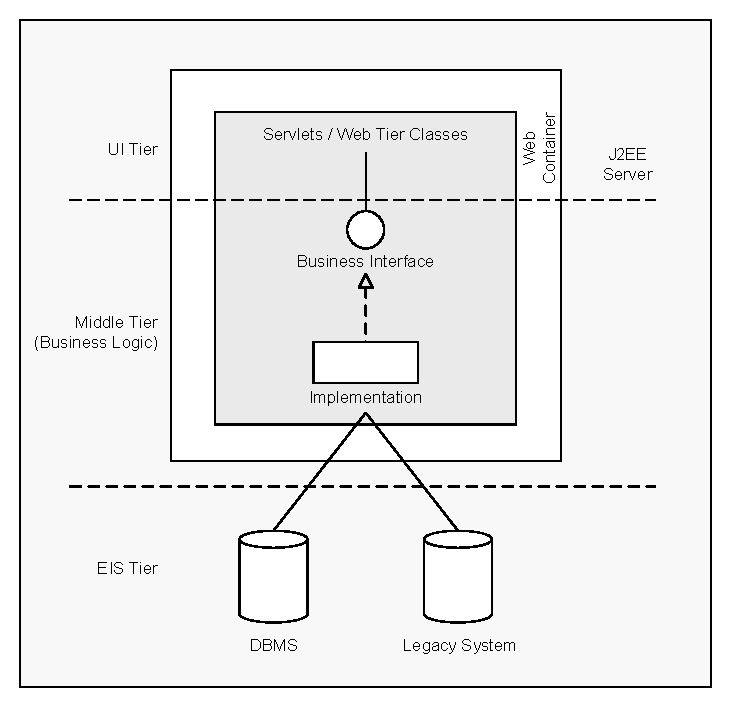
\epsfig{file=images/jee3tier.eps, width=80mm}
  \caption{The Java~\abbrev{EE} Three-Tier Model (adapted from
  \citep{j2eednd})}
  \label{fig:jee3tier}
\end{center}
\end{figure}

In Java~\abbrev{EE} world, the three-tier application tiers are called 
the \textsl{\abbrev{UI} tier}, the \textsl{middle tier} and the 
\textsl{\abbrev{EIS} tier} (for Enterprise Information System) 
\citep{j2eednd}. The Java~\abbrev{EE} three-tier model is shown in 
image~\ref{fig:jee3tier}. The tiers in this model are often 
distributed to separate machines. Each single tier can in fact be 
clustered to multiple machines to achieve maximal performance and 
throughput. Java applications wanting to be Java~\abbrev{EE} compliant 
must implement this model as a bare minimum \citep{rapidspring}.


% Presentation Tier: Model-View-Controller
% ----------------------------------------
\subsection{Presentation Tier: Model-View-Controller}
\label{toc:webdevel:threetier:presentation}

When designing the presentation tier of an application it is 
important to keep in mind the principle of \textsl{model-view 
separation}. The model-view separation principle states that the model 
(the domain representation) of the system should not have direct 
knowledge of the view objects (the presentation tier) 
\citep{applying}. The \textsl{model-view-controller} design pattern 
(\abbrev{MVC}) is a model that supports this principle, and is shown 
in image~\ref{fig:mvcmodel}.

\begin{figure}
\begin{center}
  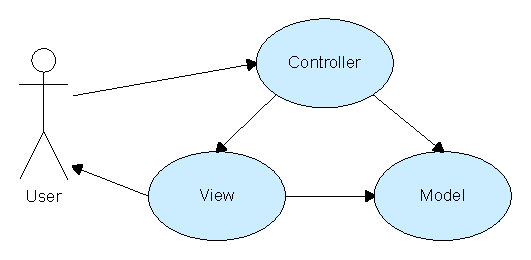
\epsfig{file=images/mvcmodel.eps, width=80mm}
  \caption{The \abbrev{MVC} Model}
  \label{fig:mvcmodel}
\end{center}
\end{figure}

The model-view-controller pattern divides the program into three 
pieces: the \textsl{model}, which contains the domain model of the 
system; the \textsl{controller}, which coordinates the actions 
performed on the system; and the \textsl{view}, which shows the 
current state of the system to the user. As shown in 
image~\ref{fig:mvcmodel}, the user of the system only gives input to 
the controller and receives output from the view objects. 
\citep{legacymvc,mvcpac}

The \textbf{model} objects contain both the state of the application 
and the core functionality of the system. Database access and 
transactions are also implemented in these components. The model 
objects offer a stand-alone access to the application data -- they 
usually do not and should not have any direct knowledge of the view or 
controller components.

The \textbf{view} objects provide a visual view of the application 
state. Everything shown to the user is rendered via the view 
components. It is important that the view components themselves do not 
contain any application logic, but only show the current state of the 
application to the user as represented by the model objects. In the 
traditional \abbrev{MVC} model, the model can inform the view whenever 
it changes so that the view can be updated. To keep the model-view 
separation in effect, this is often accomplished with the 
\textsl{Observer} pattern \citep{applying}, which keeps the model 
unaware of the actual view objects. In the optimum situation the view 
object can be easily changed to another implementation without 
touching the model or even the controller.

The \textbf{controller} controls the interactions between the user of 
the system and the model objects and selects the correct view to show. 
A standard controller in a request-based system processes the 
requests, creates the necessary model objects, performs the required 
actions on the model objects and forwards the user to a view that 
shows the results of the actions.

\abbrev{MVC} is not a new model, and it has demonstrated its 
advantages by supporting the creation of multiple views to the same 
data and allowing easy code reuse \citep{dbwebmvc}. Furthermore the 
model promotes low coupling and high cohesion (\abbrev{GRASP} 
\citep{applying}) by keeping the different aspects of software 
separate.

Although the \abbrev{MVC} model can be used as an architectural model 
for an entire application, it is often used in the presentation tier 
of a web application. In a servlet-based Java presentation tier the 
servlets act as controllers, processing input read from user. The 
input is then forwarded to the business tier of the application (the 
model). Finally, the results of the servlet actions are shown to the 
user via the view components, which are usually \abbrev{JSP} pages.


% Business Tier: Business Objects and Operations
% ----------------------------------------------------
\subsection{Business Tier: Business Objects and Operations}
\label{toc:webdevel:threetier:middle}

As discussed before, the business tier of an application contains the 
business objects and operations that represent and maintain the state 
of the system. Typically the business objects require a multitude of 
references to other business objects, helper objects and data sources. 
A common problem especially in the business tier is the configuration 
and setup of the required classes. One traditional way of configuring 
the objects is the usage of the \textsl{Singleton} design pattern 
\citep{applying}, but the pattern is not without its drawbacks. Using 
singletons leads to hard-coded dependencies to the singleton objects
and each singleton must handle its own configuration independently 
\citep{j2eednd}. 

Fortunately application frameworks provide methods for configuring the 
required objects, usually via \abbrev{XML} configuration files. An
\textsl{application context} object (also known as \textsl{registry} 
or \textsl{application toolbox}), creates, configures and manages the 
required objects. The objects can either be fetched from the 
application context by specifying their name, or they can be 
automatically set to all the objects that require them by the 
application context (see dependency injection in 
section~\ref{toc:webdevel:patterns:ioc}). This relieves the 
application developer from the burden of reading configuration files 
or creating hard-coded singleton objects.

Another commonly heard buzzword in the Java~\abbrev{EE} world is 
\abbrev{EJB}, the Enterprise JavaBeans, which is also a solution for 
the business tier. \abbrev{EJB} 2.0 defines \textsl{entity beans} that 
represent the business objects, \textsl{session beans} that represent 
the business processes and operations, and \textsl{message-driven 
beans} that coordinate tasks that involve other entity and session 
beans \citep{ejb}. However, \abbrev{EJB}s are a heavyweight technology 
with significant coding overhead \citep{usingj2ee}, and their usage is 
fully justified only when there is a requirement for a distributed 
environment. In addition, \abbrev{EJB} is the most complex technology 
in Java~\abbrev{EE} and it is very hard to test because of the 
distributed environment it requires to run \citep{j2eednd}.

\abbrev{EJB} 3.0 addresses some of the issues of previous \abbrev{EJB}
versions but it has just been published and has not yet reached the 
standard-level. Using it can therefore still be a bit risky 
\citep{modeltransejb}.



% Database Tier: Object/Relational Mapping
% ----------------------------------------
\subsection{Database Tier: Object/Relational Mapping}
\label{toc:webdevel:threetier:db}

Virtually all web software applications operate on some data that 
needs to be persisted. Most commonly the data is persisted by storing 
it to a database. Databases come in two distinct varieties: there are 
relational databases (\abbrev{RDBMS}) and object-oriented databases 
(\abbrev{ODBMS}, or \abbrev{OODBMS}). The relational databases store 
textual, numeric and binary data in rows and columns of tables. In 
contrast, object-oriented databases add data persisting capabilities 
to the host programming language itself. Even though the 
object-oriented databases would seem more suitable for object-oriented 
languages, they have not been widely adopted. For example, all 
Java~\abbrev{EE} applications are object-oriented by definition, but 
still use mostly relational databases. \citep{j2eednd,hibernateaction}

Using relational databases with object-oriented programming brings out 
a \textsl{paradigm mismatch}: object hierarchies with inheritance and 
dependencies to other objects need to be stored as row data in 
database tables. This conversion from an object-oriented world into 
the world of tables and rows is not a trivial problem to tackle. 
\citep{hibernateaction}

A common solution to this paradigm mismatch is 
\textsl{object/relational mapping}. \abbrev{ORM} is an attempt to 
automatically and transparently map the state of objects into the rows 
of a relational database and back into objects. \abbrev{ORM} often 
requires guidance to govern the transformation. This is provided by 
supplying and maintaining metadata alongside with the actual objects. 
Although this implies a certain overhead for the developers, it 
eliminates the need to write simple create, read, update and delete 
(\abbrev{CRUD}) queries. \citep{hibernateaction}

In addition to this solution, Enterprise JavaBeans provide their own 
data persisting capabilities \citep{ejb}. However, as discussed in the 
previous section, \abbrev{EJB}s do have their disadvantages and a more 
lightweight approach can be more suitable for a non-distributed 
program \citep{j2eednd}.



%%%%%%%%%%%%%%%%%%%%%%%%%%%%%%%%%%%%%%%%%%%%%%%%%%%%%%%%%%%%%%%%%%%%
% Design Patterns
%%%%%%%%%%%%%%%%%%%%%%%%%%%%%%%%%%%%%%%%%%%%%%%%%%%%%%%%%%%%%%%%%%%%
\section{Design Patterns}
\label{toc:webdevel:patterns}

There is no single, clear definition for \textsl{design patterns}. 
\cite{patternj2ee} defined design patterns as "\textsl{recurring 
solutions to standard design problems in contexts}." The basic idea 
behind all the different definitions is that a design pattern 
describes a common problem and a general solution that can be applied 
to the same problem in different contexts. A design pattern is 
therefore a known and widely used solution to a recurring problem. 
Design patterns evolve from the solutions that are used, they are not 
invented \citep{applying}.

In software design, there are patterns in multiple levels. General 
Responsibility Assignment Software Patterns (GRASP \citep{applying}) 
describe fundamental object design and responsibility assignment 
practices. These patterns explain basic ideas such as who should 
create objects, how they should interact with each other and what kind 
of references objects should have to each other in object hierarchies. 
Another group of design patterns is called the Gang-of-Four 
(\abbrev{GoF}) patterns \citep{applying}. The \abbrev{GoF} patterns 
apply to the architecture level of a program. The well-known 
\textsl{Observer} pattern, for example, describes how a data item can 
notify different components (the observers, or listeners) of changes 
without being tied to their implementations.

This section describes several patterns that apply to web development. 
One of them, the model-view-controller pattern, was already introduced 
in section~\ref{toc:webdevel:threetier:presentation}.



% Front Controller
% ----------------------------------------
\subsection{Front Controller}
\label{toc:webdevel:patterns:front}

The front controller is a design pattern for the presentation tier. It 
defines a single entry point for requests which enables common control 
and request handling for the entire application \citep{patternj2ee, 
corej2eepat}. Centralised request processing ensures that no request 
processing logic is intermingled with the application views. Sharing 
the common entry point also enforces a uniform request processing 
logic for the application.

The front controller pattern contains four different object types:
\begin{description}
  \item[Controller] Provides the entry point for all web application 
  requests. The controller uses \textsl{helpers} to process the 
  request and forwards the results to the \textsl{dispatcher}. The 
  controller is typically a Java servlet.

  \item[Dispatcher] Manages the \textsl{views} and the navigation 
  between them. The dispatcher selects the proper view and shows it to 
  the user. The dispatcher can be encapsulated in the controller or it 
  can be a separate component.

  \item[Helper] Responsible both for helping the controller process 
  the different requests and for providing the views with the 
  information they require.

  \item[View] Used to show the results of the request to the user. The 
  views are often \abbrev{JSP} pages, which do not contain any 
  business logic. All information shown on the views is obtained from 
  the helpers.
\end{description}


% Inversion of Control
% ----------------------------------------
\subsection{Inversion of Control}
\label{toc:webdevel:patterns:ioc}

Traditional software library reuse consisted of the developer writing 
a main program which calls upon the interfaces provided by the reused 
software components. While this works well with libraries that serve a 
single purpose and have a clear interface, it also means that all 
developers must develop and maintain the actual structure of their 
applications.

The inversion of control (\abbrev{IoC)} design pattern provides an 
alternative approach to program control. With \abbrev{IoC}, the reused 
software library (most often an entire framework) has an application 
context object that maintains the control of the application and calls 
on the operations defined by the developer 
\citep{fweqcomppat,parviainen}. The \abbrev{IoC} pattern embodies the 
Hollywood principle: "\textsl{don't call me, I'll call you}" 
\citep{j2eednd}.

Most current frameworks work according to the principle of inversion 
of control. By leaving the structure of the application to the 
framework, the developer can concentrate on implementing the actual 
business logic.

There are two main types of inversion of control: \textsl{dependency 
lookup} and \textsl{dependency injection} \citep{rapidspring}. These
are described below.

\begin{description}
\item[Dependency Lookup] With dependency lookup, the application 
context provides each managed class with a reference to the context. 
The objects can then use the \abbrev{API} methods of the context to 
find the resources they need.

\item[Dependency Injection] Another approach to managing object 
configuration is dependency injection. In this approach the context 
does not supply the managed object with a reference to itself, but 
instead provides the required references directly. This means that the 
responsibility for dependency lookup is wholly on the application 
context, and the objects are freed from dependencies on the 
application context \abbrev{API}s.
\citep{rapidspring}

There are two common ways to accomplish dependency injection. With 
\textsl{constructor injection}, the settings are passed via the 
constructor of the object. In \textsl{setter injection}, the 
configuration is set via JavaBean properties\footnote{JavaBean 
properties are class fields that have standard getters and setters. 
For example, to implement a JavaBean property \codefn{colour}, the 
methods \codefn{getColour()} and \codefn{setColour()} must be 
defined.}.

\end{description}


% AntiPatterns
% ----------------------------------------
\subsection{AntiPatterns}
\label{toc:webdevel:patterns:antipatterns}

Although design patterns, when applied correctly, can dramatically 
enhance the software design quality, they can degenerate to 
\textsl{AntiPatterns} when used in the wrong context or as a solution 
to the wrong problem. According to \cite{antipatterns}, an AntiPattern 
is "\textsl{a literary form that describes a commonly occurring 
solution to a problem that generates decidedly negative 
consequences}." When discussing design patterns, it is important to 
realise that enforcing the usage of wrong patterns can lead the 
project to disaster.

As the software engineering industry develops, from time to time 
certain solutions are presented as the "silver bullet" that will solve 
all software engineering problems at one go. These software fads 
include \textsl{structured programming}, which was supposed to improve 
productivity and remove software defects; \textsl{networking} 
technologies, which were supposed to make all systems interoperable; 
and \textsl{object orientation}, which was supposed to solve the 
problems of adaptability and make software highly reusable. While 
these solutions are not bad, they do not have an answer to all the 
problems in the field of software engineering. Believing the hype 
around new software development methods is one of the key factors in 
turning the methods into AntiPatterns. \citep{antipatterns}

Several well-known AntiPatterns include \textbf{The Golden Hammer}, 
which happens when a familiar technology or concept is applied to 
virtually all software problems without regard to its suitability; and 
\textbf{Cut-and-Paste Programming}, which describes the maintenance 
nightmare situation when code has been reused by copying source code 
statements. \citep{antipatterns}


%%%%%%%%%%%%%%%%%%%%%%%%%%%%%%%%%%%%%%%%%%%%%%%%%%%%%%%%%%%%%%%%%%%%
% Artifact Generation
%%%%%%%%%%%%%%%%%%%%%%%%%%%%%%%%%%%%%%%%%%%%%%%%%%%%%%%%%%%%%%%%%%%%
\section{Artifact Generation}
\label{toc:webdevel:artifactgen}

Many programming techniques and tools require information in their own 
configuration files and in a specific format. Others, like 
\abbrev{RMI} and \abbrev{EJB}, demand the creation of interfaces that 
follow their respective conventions. Creating and maintaining 
supporting code and configuration files is a tedious and error-prone 
task. \cite{j2eednd} reckons that it is impossible to create and 
maintain \abbrev{EJB} 2.0 entity beans by hand when using 
container-managed persistence (\abbrev{CMP}), because they are far too 
complex.

To tackle the issues with supporting code and configuration files, 
tools that generate the required artifacts automatically have been 
created. Code generators can create all the classes required by the 
\abbrev{EJB} architecture from a single file. Configuration file 
generators can create framework configuration files from source code 
that is annotated with special annotations. These tools help reduce 
the amount of code required and remove the separation between the 
definition of an object and the required supporting configuration.

Code generation in itself can mean at least two things: generating 
code automatically from special markup; or generating code from formal 
specifications. While code generation from formal specifications can 
be seen to provide the most benefits, such as dramatically reduced 
development effort and provably correct implementation (with respect 
to specifications) \citep{codegenreq,exploringcodegen}, many of these 
benefits apply to code generation from markup also. Automatic 
configuration file generation ensures that there are no syntactical 
errors in the files. Extracting interfaces automatically eases the 
creation and maintenance of \abbrev{EJB} entity beans \citep{j2eednd}.


%%%%%%%%%%%%%%%%%%%%%%%%%%%%%%%%%%%%%%%%%%%%%%%%%%%%%%%%%%%%%%%%%%%%
% Summary
%%%%%%%%%%%%%%%%%%%%%%%%%%%%%%%%%%%%%%%%%%%%%%%%%%%%%%%%%%%%%%%%%%%%
\section{Summary}
\label{toc:webdevel:summary}

This chapter presented several key concepts in modern web software 
development. The introduction to web development started with the
\abbrev{JSP} models, which are now taken out of \abbrev{JSP} 
specifications. However, the \abbrev{JSP} model 2 can still be seen as 
a valid starting point for designing web applications.

Section~\ref{toc:webdevel:frameworks} identified the need for using 
frameworks in web development. Frameworks provide a consistent 
structure to the application as well as supplying robust and tested 
functionality.

The Java~\abbrev{EE} platform was introduced in 
section~\ref{toc:webdevel:javaee}. Java~\abbrev{EE} provides a set of 
common interfaces for building enterprise applications. Although it is 
widely used, many projects have produced unduly complex systems when 
using Java~\abbrev{EE} in the wrong way.

Section~\ref{toc:webdevel:threetier} presented the three-tier 
application model, which consists of the \textsl{presentation tier}, 
the \textsl{business tier} and the \textsl{database tier}. This model 
is the most typical enterprise application model and is the smallest 
model that can be considered Java~\abbrev{EE} compliant. Software 
needs were identified for each of the three tiers. For the 
presentation tier, a model-view-controller framework is recommended. 
In business logic tier, a business object framework is required. For 
the database tier, support for the object/relational mapping is needed.

In section~\ref{toc:webdevel:patterns}, some important design patterns 
for web development were introduced. These include the \textsl{front 
controller} pattern, which is used as a single point-of-entry in the 
presentation tier of a web application; and the \textsl{inversion of 
control} pattern, in which a framework is responsible for program 
control.

Finally, section~\ref{toc:webdevel:artifactgen} described the need for 
automatic generation of various software artifacts. Automatic artifact 
generation reduces implementation effort and removes syntactical 
errors from the generated artifacts.

